\documentclass{standalone}
\usepackage{tikz}
\usepackage{pgfplots}
\pgfplotsset{width=32cm,height=18cm,compat=1.3}
\pgfplotsset{every tick label/.append style={font=\Huge}}
\usepackage{filecontents}
\usepgfplotslibrary{fillbetween}

\usetikzlibrary{patterns}

%\definecolor{citrine}{rgb}{0.89, 0.82, 0.04}
%\definecolor{arylideyellow}{rgb}{0.91, 0.84, 0.42}
%\definecolor{bronze}{rgb}{0.8, 0.5, 0.2}

\definecolor{color1}{RGB}{230,97,1}
\definecolor{color2}{RGB}{253,184,99}
\definecolor{color3}{RGB}{178,171,210}
\definecolor{color4}{RGB}{94,60,153}

\begin{document}
	\centering
		\vspace{1.5em}
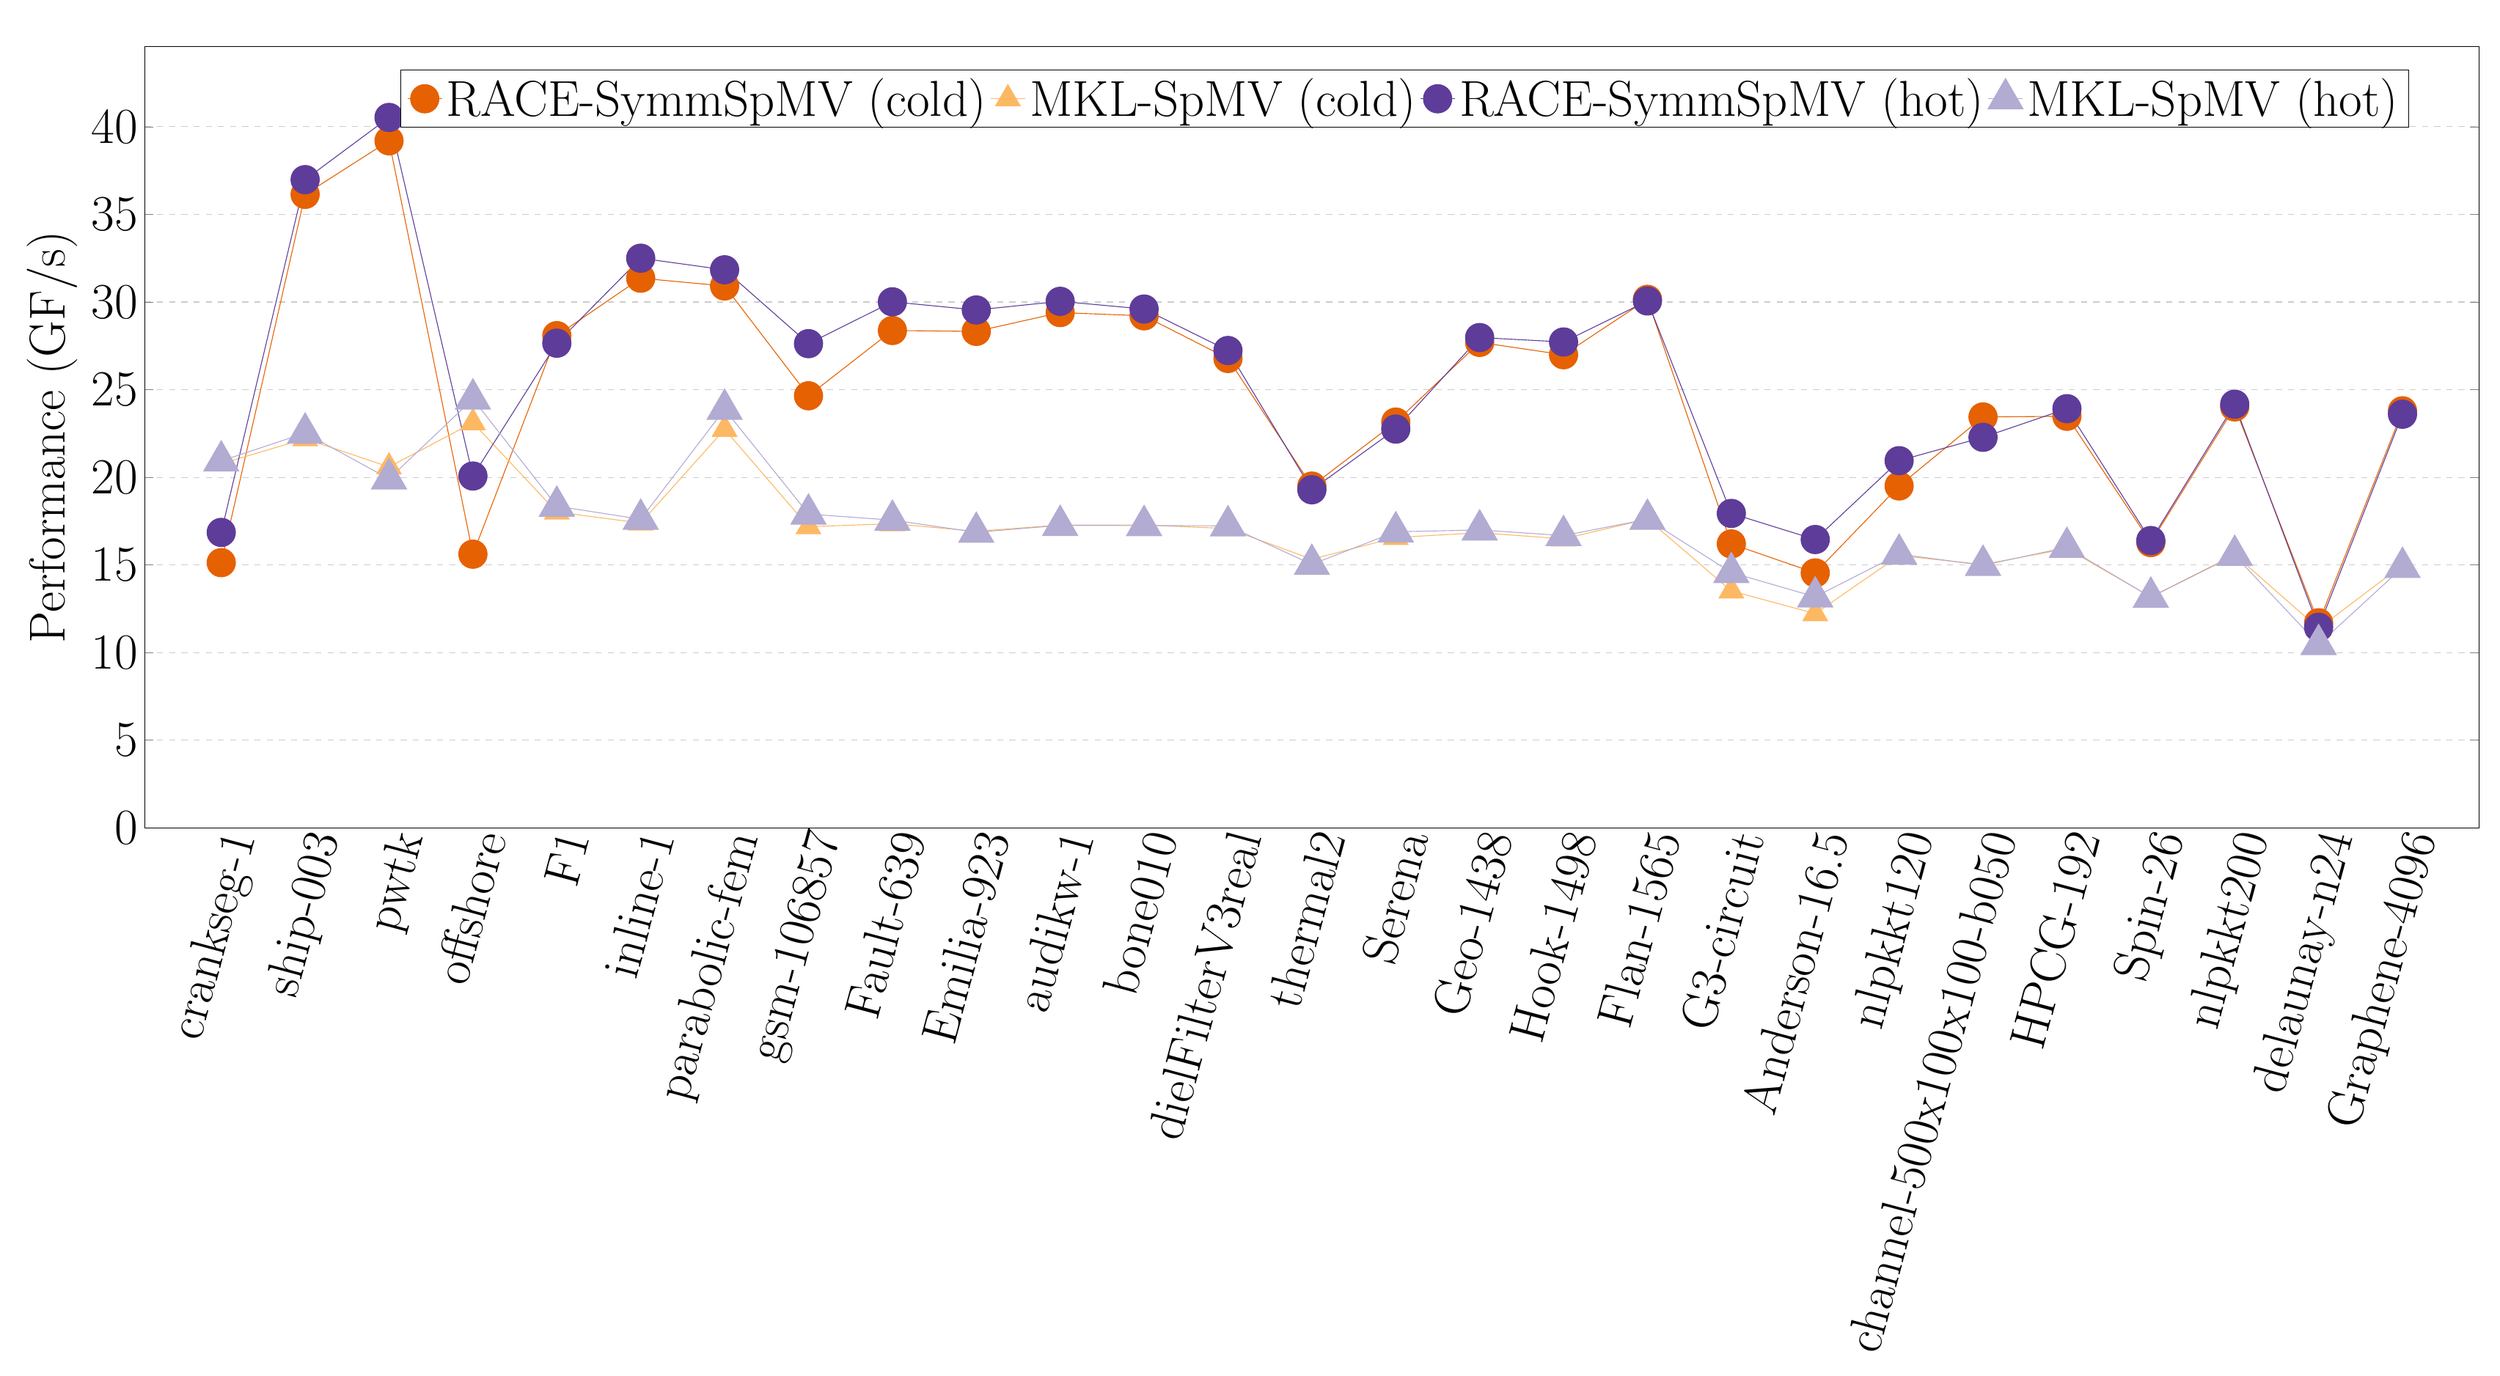
\begin{tikzpicture}
		%	\node at (13.25,15) {\LARGE{}};
			\begin{axis}[
		%	xmin=0.25, xmax=7.25,
			ymin=0, %ymax=3.25,
			xtick={1, 2, 3, 4, 5, 6, 7, 8, 9, 10, 11, 12, 13, 14, 15, 16, 17, 18, 19, 20, 21, 22, 23, 24, 25, 26, 27, 28, 29, 30, 31},
		%	ytick={0,0.5,1,1.5,2,2.5,3},			
			xticklabels={crankseg-1, ship-003, pwtk, offshore, F1, inline-1, parabolic-fem, gsm-106857, Fault-639, Emilia-923, audikw-1, bone010, dielFilterV3real, thermal2, Serena, Geo-1438, Hook-1498, Flan-1565, G3-circuit, Anderson-16.5, nlpkkt120, channel-500x100x100-b050, HPCG-192, Spin-26, nlpkkt200, delaunay-n24, Graphene-4096},
			width  = 42cm,
			height = 15.12cm,
			major x tick style = transparent,
			%	minor ytick={1, 5, 10, 15, 20, 25, 30 ,35,40},
			grid = minor,	
			%add_bar_commands
			ymajorgrids = true,
			grid style={dashed, gray!40},
			ylabel = {\Huge{Performance (GF/s)}},
		%	symbolic x coords={Graphene-2048-2048, Graphene-4096-4096, Spin-24-24-24},
			x tick label style={rotate=75, anchor=north east, inner sep=0mm, font={\Huge}},
			tick label style={font={\Huge}},
			scaled y ticks = false,
			enlarge x limits=0.035,
			legend cell align=left,
			legend style={font=\Huge},
			legend columns=-1,
			legend style={
				%at={(1,1.05)},
				%anchor=south east,
				%column sep=1ex,
				legend pos=north east
			},
			%spl_legend_code
			title= {\Huge\scalebox{1.5}{{}}}
			]

\addplot[name path=1, mark=*, mark size=7pt, mark options={color1}, draw=color1 ] plot coordinates{(1,15.130207) (2,36.140175) (3,39.194893) (4,15.613967) (5,28.080251) (6,31.356939) (7,30.913152) (8,24.649314) (9,28.372987) (10,28.323231) (11,29.396679) (12,29.210280) (13,26.778583) (14,19.496395) (15,23.148677) (16,27.696097) (17,26.990050) (18,30.152423) (19,16.199662) (20,14.545610) (21,19.505411) (22,23.441453) (23,23.480804)  (24,16.275497) (25,24.014713) (26,11.700657) (27,23.793009)};
\addplot[name path=4, mark=triangle*, mark size=7pt, mark options={color2}, draw=color2 ] plot coordinates{(1,20.769206) (2,22.199856) (3,20.590162) (4,23.111813) (5,18.019958) (6,17.389334) (7,22.738380) (8,17.180456) (9,17.354518) (10,16.918081) (11,17.275771) (12,17.277571) (13,17.077006) (14,15.326098) (15,16.566454) (16,16.836613) (17,16.487552) (18,17.619697) (19,13.517244) (20,12.222770) (21,15.527179) (22,15.026985) (23,15.929758)  (24,13.177933) (25,15.587776) (26,11.374282) (27,14.997639)};

\addplot[mark=*, mark size=7pt, mark options={color4}, draw=color4 ] plot coordinates{(1,16.854992) (2,36.979831) (3,40.528888) (4,20.072225) (5,27.650065) (6,32.497825) (7,31.837543) (8,27.622948) (9,30.008732) (10,29.544466) (11,30.038410) (12,29.598056) (13,27.233392) (14,19.287252) (15,22.750551) (16,27.971316) (17,27.719366) (18,30.058614) (19,17.938689) (20,16.449635) (21,20.948219) (22,22.279768) (23,23.914583) (24,16.392259) (25,24.170988) (26,11.440436) (27,23.598034)};
	%addplot cmd

\addplot[mark=triangle*, mark size=10pt, mark options={color3}, draw=color3 ] plot coordinates{(1,20.929816) (2,22.524163) (3,19.912094) (4,24.466454) (5,18.352351) (6,17.607485) (7,23.879831) (8,17.902683) (9,17.554796) (10,16.865151) (11,17.257002) (12,17.248342) (13,17.231437) (14,15.033728) (15,16.890168) (16,16.996224) (17,16.676041) (18,17.605660) (19,14.566514) (20,13.180425) (21,15.616247) (22,14.979805) (23,16.001894) (24,13.160505) (25,15.547540) (26,10.461543) (27,14.860118)};

	\legend{RACE-SymmSpMV (cold),  MKL-SpMV (cold), RACE-SymmSpMV (hot), MKL-SpMV (hot)}

	\end{axis}			
\end{tikzpicture}

\end{document}

